%!TEX root = ../LastNameI-[RnD-MT]Report.tex

\chapter{Introduction} 
Robot manipulation is an important field of research in robot technology. In the past years, there has been a large and varied growth in the field of robotic systems, concerning its tasks. Within industries around the world, robots perform a variety of manipulation tasks on a daily basis. They lift heavy objects, move with high speed, and repeat complex performances precisely. The field of robot manipulation can be further sub-classified to kinematics and dynamics, motion planning and control and also higher mathematics. 
\par
Kinematics studies the possible motions of the robot without taking into consideration the forces that are necessary to produce that motion. There has been substantial research effort in the field of kinematics in-order to develop a general solution to the inverse kinematic problems. The major drawback in dealing with these problems is the situation of arising singular configurations in robots. Intuitively for a standard six joint industrial manipulator, these configurations can be visualized as incapability of achieving motion in a particular direction irrespective of its movements in its joints. The workspace of robots is thus limited by singularities. From the mathematical point of view, kinematic singularity can be made precise in terms of rank loss of Jacobian matrix \cite{donelan2010kinematic}. This can be interpreted as the change in instantaneous number of degrees of freedom of the robot \cite{donelan2010kinematic}. 
%in a standard six joint industrial manipulator, the robots are incapable .  	
%They lift heavy objects, move with high speed, and repeat complex performances precisely.  Robots can perform several tasks such as picking and placing objects, welding, paint spraying etc. which commonly found in industries\cite{}. They also perform domestic household tasks such as floor cleaners, The robot arm also called as robotic manipulators can perform tasks where the movements of the arm can be adapted/mimicked to that of the human arm.

%\color{orange}Kinematics is the study of all the possible motions of a robot which is a branch of classical mechanics that describes the movements of points, objects, and group of bodies without considering the interactions of motions and forces eg via inertia ~\cite{wikipedia}. \color{black}
%The change in the instantaneous number of degrees of freedom indicates that the robot manipulators enter into  kinematic singularity configurations\cite{donelan2010kinematic}. From the mathematical point of view, kinematic singularity can be made precise in terms of rank loss of Jacobian matrix. \cite{donelan2010kinematic}\\ 
The main objective of the research aims at extending the already available Popov Vereschchagin hybrid dynamics solver to detect the singularities occurring at the runtime or to detect if it is close to singularity. Popov Vereschchagin is a domain specific solver which computes control commands based on constraints imposed on them. The downside of this solver is its inability to determine runtime singularity. The solver only considers the robot's dynamics and therefore is unaware of the concept of kinematic Jacobians. Hence, the ``traditional`` means of singularity detection do not apply. This instigates that there is necessity to detect singularity that rely on the dynamics primitives available in the existing solver. The aforementioned reasons indicate the prerequisite to extend the solver to solve and detect for dynamic singularities.
\par
The report is structured as follows. Firstly, chapter \ref{SOA} provides required background and technical soundness in understanding the field of rigid body systems and their dynamics. This is followed by explaining the necessary state of the art. Main focuses are on kinematic singularities, task specifications such as Whole Body Control, Stack of tasks etc. Chapter \ref{Problem statement} address the problem statement of the research. Chapter \ref{PVS} gives a comprehensive overview of the Popov Vereschchagin solver. Followed by chapter \ref{Approach} and \ref{ER} outlines the methodology and the experiments conducted to evalaute the solutions to the problem of detecting singularities. Finally, the conclusion and the future reference to this project is stated in chapter ~\ref{conclusion}.

\section{Motivation} \label{Motivation}

\begin{figure}[h!]
	\centering
	\begin{minipage}{0.45\textwidth}
		\centering
		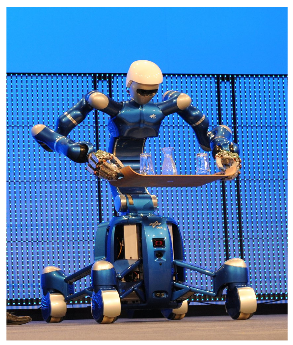
\includegraphics[width=0.8\textwidth]{images/mot1} % first figure itself
		\caption{Situation depicting robot carrying heavy tray \cite{robottray}}
		{Case1: Necessity to avoid singular configuration}
	\end{minipage}\hfill
	\begin{minipage}{0.45\textwidth}
		\centering
		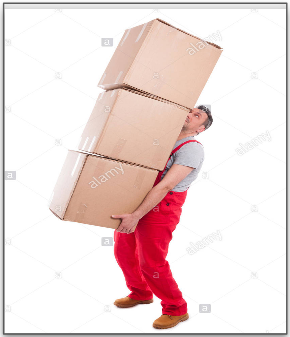
\includegraphics[width=0.82\textwidth]{images/mot2} % second figure itself
		\caption{Situation depicting human carrying heavy box \cite{mot1}}
		{Case2: Necessity to utilize singular configuration}
	\end{minipage}
\end{figure}
%	\begin{figure}[h!]
%		\centering
%		
\includegraphics[scale=0.45]{images/motivation}		
%		\caption{Situations depicting }
%	\end{figure}
Depending on the tasks performed by the robot, two situations could be of concern. The first situation is avoiding and the second is to exploit (utilize) singular configurations in the robot. 


Considering an example, referring to the case in the human body, where human's posture while in standing (stretched legs) position. Evaluation on the level of forces, this assists by allowing all the forces to be applied on the joint constraints of the legs while reducing the forces applied to the muscles. An important motive behind the problem is to utilize the opportunity of exploiting singularities in the context of tasks and which allows the robot to minimize energy consumption. 
%An example would be . 


There are various reasons for the occurrence of singularities. The importance of singularities from an engineering perspective are mentioned below  ~\cite{abdolmalaki2017geometric}:


In many cases, robot manipulators are required to perform tasks under contact with objects or environment. The endpoint of the manipulator is in contact with the environment. We have several examples describing the above situation, one of them can be by considering a robot which is required to push heavy loads and is also in contact with the object. A mechanical advantage can be realized for eg: load-bearing capacity \cite{abdolmalaki2017geometric}. Hence for above scenario, it is best to seek singularity. 


A robot's task is described usually in its task space. In order to provide significant application efficiency and flexibility to a robotic operation a direct implementation of a task level controller is performed. However, the existence of singularities is the crucial problem in the application of task level controllers \cite{Clara2012}. While approaching singular configuration, the task level controllers may generate high joint torques. The outcome is large errors and in instability in the task space \cite{tan2004singularity}. In general a 6 degrees of freedom (DOF) task, such as welding will require the robot to avoid singular configuration in-order to perform the task. Also near the singular configurations, a large movement of joint variables may result in small motions of the end–effector \cite{donelan2007singularities}. In these cases, it is necessary to avoid singularities.


These instances provide an insight into the problem, where we distinguish into mechanism and policy where the mechanism is to detect singularities at the runtime and also the policy is to know how to exploit this knowledge. This provides the best situation in order to avoid or utilize singularity.


The above given examples are extremely dependent on the type of robot task. The question would be how to make use of them in our applications. Here, the focus is on how to ensure that the singularity does not influence the task. Based on the type of the singularity, for eg. internal singularity can be avoided by control. But workspace singularities require the help of mobile base. Therefore with this knowledge, we will be able to derive valuable information about how to handle them ~\cite{Buss2004}.


%\section{Challenges and Difficulties}
%\section{Problem Statement}
	